\chapter{Prototypen} 
In diesem Kapitel entstehen Prototypen, die Renew schrittweise modularisieren bis die Applikation den größten Teil ihre Funktionalität auf dem Modulpfad betreiben kann. 


Für die Umsetzung werden zuerst Anforderungen erfasst, die der modularisierte Renew Prototyp erfüllen muss um unserer Vision der Implementation zu entsprechen. Infolgedessen entsteht ein Implementierungsplan sowie ein Prototyp. 

%Anforderungen an System 
\section{Anforderungen} \label{sec:anforderungen}
Im Kern der Modernisierung von Renew liegt die Anpassung von Renew an das Modulsystem von Java und dessen Anforderungen an Applikationskomponenten. Aus den Renew Plugins sollen explizite Module entstehen, die auf dem Modulpfad betriebsfähig sein müssen. Die Drittanbieter-Bibliotheken sollen mit in den Modulpfad aufgenommen werden und als automatische Module ihre Aufgabe erfüllen. Zusätzlich darf die Migration und damit verbundene Anpassung und Aufbereitung der Mängel die Kommunikation sowie interne Funktionsweise von Renew nicht verändern. Dementsprechend soll garantiert werden, dass die darunter liegende theoretische Grundlage in Takt bleibt. 

%was soll der Prototyp leisten 
\subsection{Interaktion}
Der erste modulare Renew Prototyp soll mit einer minimalen Plugin Anzahl auf dem Modulpfad betriebsfähig sein und eine Möglichkeit bieten Petrinetze zu erstellen, zu simulieren und zu serialisieren. Das heißt, es muss eine UI zu sehen sein, die mit den nötigen Werkzeugen und der darunter liegender Logik ausstattet ist. 

\subsection{Projektstruktur}
Für die Umsetzung des modularen Renew's wird für jedes Plugin eine moderne Projektstruktur benötigt, die den Inhalt entsprechend dem etablierten Maven Standardverzeichnislayout auf Java Module und die dafür benötigten Ressourcen aufteilt. 

\subsection{Entwicklungsumgebung} 
In der existierenden Renew Entwicklungsumgebung werden alle Plugin Projekte durch eine versteckte \textit{.project} beschrieben. Das heißt, der Klassenpfad und die binden der Codebausteine geschieht versteckt und für den Entwickler schwer zugänglich. Es liegt ein weiter und verschachtelter Weg der Eclipse Konfiguration-UI, die sich mit der Zeit verändern kann. Dieser Umstand wurde von mir im letzten Projekt beobachtet und kostete Zeit für alle Projektteilnehmer, da die Universitätsrechner strikten Rechten unterliegen, die keine eigen Eclipse Entwicklungsumgebung aufsetzen lässt. Darüber hinaus ist die Konfiguration von Renew in anderen Entwicklungsumgebungen wie IDEA oder Netbeans mit der \textit{.project} Konfigurationsdatei nicht möglich.
\bigbreak

Um eine Entwicklungsumgebung unabhängige Konfiguration anzulegen wird ein neues Werkzeug benötigt. 

\subsection{Packaging}
Da die Umstrukturierung von Renew an das Modulsystem durchgeführt werden muss, muss das für die Kompilation und Verpacken der Codebasis verantwortliche Werkzeug die Veränderung miterleben. 


Renew benutzt zur Zeit das \textit{Apache Ant} Werkzeug, dass alle Plugins kompiliert und in einer ausführbare Form bringt. Dieses ist in Jahre gekommen und enthält wesentlich geringeren Funktionsumfang gegenüber der Aktuellen Konkurrenz, wie Maven und Gradle. Diese bieten eine Abhängigkeitsverwaltung, konfigurierbare Plugins und sogar eine Programmiersprache. Im Gesetz zu der aufgeblasenen XML-Konfiguration von Ant, beherrschen die modernen \textit{build} Werkzeuge die Komplexität durch den \textit{Convention over Configuration} Ansatz und flexiblen Ausdrucksweisen. 
\bigbreak

Die minimalen Version von Renew soll sich an einem modernen \textit{build} Werkzeug bedienen und eine Ausführbares Ergebnis erzielen.


% wie setze ich die Anforderungen um 
\section{Spezifikation}
Um die Anforderungen umzusetzen, wird die erarbeitete minimale Version isoliert, umstrukturiert und mit dem Gradle \textit{build} Werkzeug für das Arbeiten in der Entwicklungsumgebung IDEA aufgerüstet. Da Gradle die Verwaltung des Projekts sowie das Kompilieren und Erstellen von ausführbaren Paketen übernehmen kann, ist es eine gute Wahl für das Aufsetzen einer modernen modularen Projektstruktur mit einem aufstrebenden Werkzeug. 


Dafür muss das bestehende Ant \textit{build} System analysiert und mit dem Gradle Werkzeug aufgebaut werden. Dieses soll so gut wie möglich die bestehende Drittanbieter-Bibliotheken verwalten, Module kompilieren und die benötigten Erweiterungen, wie das JavaCC Werkzeug, unterstützen.  
\bigbreak

Nachdem die Projektstrukturen die passende Form angenommen haben, müssen die Projekt Abhängigkeiten analysiert und innerhalb der \textit{module-info.java} aufgenommen werden. 
\bigbreak

Zu Letzt entsteht ein bekannte Ordnerstruktur mit Drittanbieter-Bibliotheken, Plugins und Konfigurationsdateien, die  über den \textit{Plugin Manager} verwaltet werden. 

% was werde ich tun um die Spezifikation zu erfüllen 
\section{Entwurf}
Der Entwurf berücksichtigt die schrittweise Migration und lässt die Renew Applikation während der Gesamtmigration betriebsfähig bleiben. Das heißt, Plugins auf den Klassenpfad sowie Modulpfad können nahtlos mit einander kommunizieren und ihre Funktion während der Migration weiterhin erfüllen.   
\bigbreak

% Grobe darstellung der Projketstruktur als baum 
Für den ersten Prototypen wird zuerst eine, Projektstruktur erstellt die für jedes Plugin Projekt die Möglichkeit bieten soll aus mehreren Modulen zu bestehen. Dafür wird eine Struktur \ref{fig:projektstruktur} erstellt, die im Java Verzeichnis alle Module bündelt, die über den Modulnamen disjunkt von einander verwaltet werden. Nichtsdestotrotz gehören sie zum gleichen Projekt und teilen unter sich das Ressourcen Verzeichnis, das im weiteren Verlauf zum erstellen der ausführbaren Pakete benötigt wird.

\begin{figure}[h!]
  \centering
  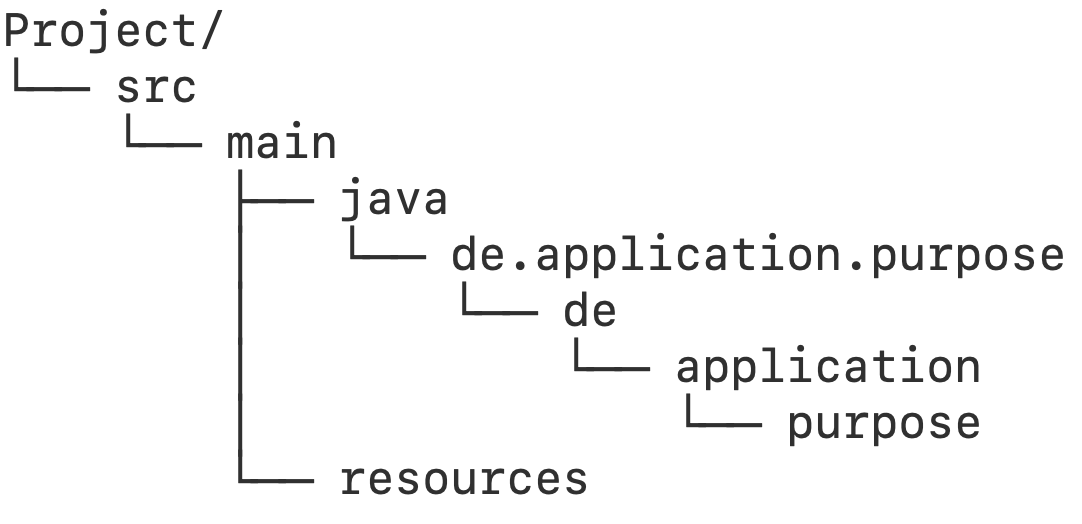
\includegraphics[width=0.6\textwidth]{material/images/project-structure.png}
  \caption{Projektstruktur}
  \label{fig:projektstruktur}
\end{figure}
       
% Wie das Gradel build system alles zusammenhalten. 
Nachdem die Projektstruktur unseren Wünschen entspricht, muss diese in der Gradle Konfigurationsdateien verankert werden. Hierfür halten wir für jedes Projekt die Projektstruktur und dessen Abhängigkeiten in der \textit{build.gradle} Konfigurationsdateien fest, indem wir Java- sowie Ressourcen-\textit{sourceSets} definieren und Projekt sowie Drittanbieter-Bibliotheken Abhängigkeiten für den  Kompilation-Pfad bestimmen.

\begin{figure}[h!]
  \centering
  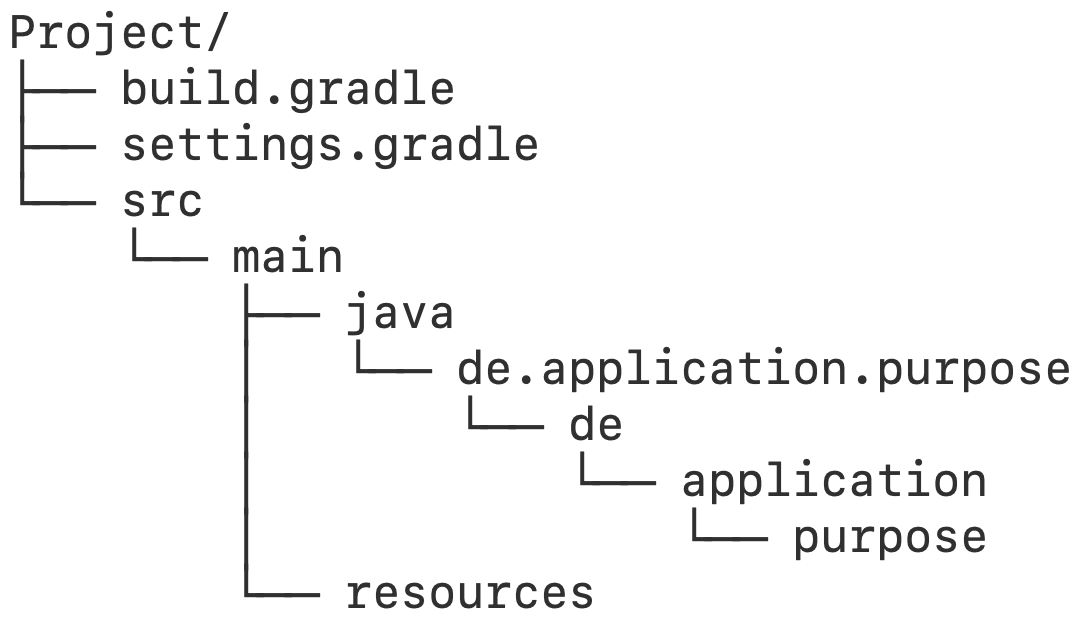
\includegraphics[width=0.6\textwidth]{material/images/gradle_project.png}
  \caption{Gradle Konfiguration}
  \label{fig:gradle_project}
\end{figure}

 Die oben genannten Schritte müssen für jedes Projekt, das für die minimal Version von Renew auserwählt wurde durchgeführt und im Anschluss über die entsprechende Entwicklungsumgebung  validiert werden. Wenn diese alle Klassen und die benötigten Abhängigkeiten finden und kompilieren kann, haben wir alle Projekte richtig strukturiert, definiert und mit einander sauber verbunden. In diesem Zustand ist die komplette Struktur des Projekts innerhalb Gradle verpackt und kann von jeder Entwicklungsumgebung ausgelesen werden. 


% Modualisierungsiddee wie ich vorgehn werden(BottomUP). 
Da jetzt eine lauffähige minimale Renew Version für den Klassenpfad erstellt werden kann, ist es Zeit diese zu Modularisieren und die einzelnen Plugins auf den Modulpfad zu migrieren. Dafür werde ich den in dem Kapitel Migration \ref{sec:bottomUP} vorgestellten \textit{bottom up} Ansatz verwenden. 

\begin{figure}[h!]
  \centering
  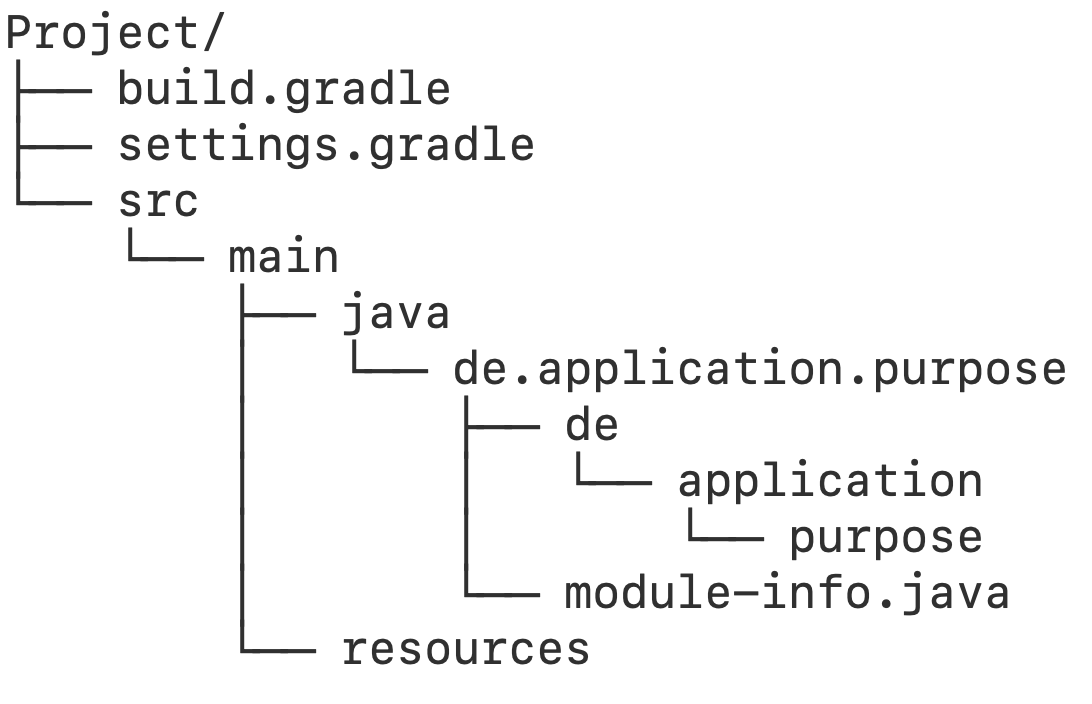
\includegraphics[width=0.6\textwidth]{material/images/module_project.png}
  \caption{Modulumwandlung}
  \label{fig:module_project}
\end{figure}

Zuerst werden die Drittanbieter-Bibliotheken, wie \textit{log4j}, auf den Modulpfad als automatische Module eingebunden und werden somit aus den Klassen- sowie Modulpfaden für die Nutzung zugleich erreichbar sein. Anschließend werden Plugins als explizite Module migriert, die keine Plugin Abhängigkeiten besitzen und aus dem Modulpfad keine Zugriffe auf den Klassenpfad ausführen, wie zum Beispiel das \textit{Util} Plugin. 
Damit diese auf dem Modulpfad ausführbar sind, werden sie durch eine \textit{moduel-info.java} Konfigurationsdatei erweitert. Diese muss sich im Stammverzeichnis des Moduls befinden wie in der Abbildung \ref{fig:module_project} dargestellt und deklariert die benötigten automatischen Module. In den nächsten Schritten werden Plugins Schritt für Schritt auf den Modulpfad migriert, indem für jedes Plugin eine eigene \textit{module-info.java} Konfigurationsdateien angelegt wird, in der sich ihre Abhängigkeiten auf automatische Drittanbieter-Module sowie explizite Plugin-Module befinden.


Dieses Vorgehen wird solange durchgeführt bis jedes Plugin sich auf dem Modulpfad befindet. 


\section{Umsetzung}


\subsection{Umstrukturierung}
 % projektstruktur anpassen
 	% split packages 
 	% resources am falschen Ort 
 	% andere Sprachen auser Java 

	Für die Umsetzung der Anforderungen und des Entwurfs wird zuerst die Projektstruktur jedes Plugins angepasst. Dafür wird die Struktur jedes Plugins analysiert, umstrukturiert und im weiteren Verlauf von Mängeln befreit. In den meisten Fällen werden \textit{split pakages} und gemischte Strukturen innerhalb der Codebasis erwartet.
\bigbreak

	Zuerst wird eine grobe Maven Projektstruktur erstellt, in dem sich zusätzlich ein Plugin Wurzelverzeichnis befindet. Anschließend migriert man die Codebasis in das Plugin Wurzelverzeichnis, welches den neuen Plugin Namen trägt.

	\begin{figure}[h!]
	  \centering
	  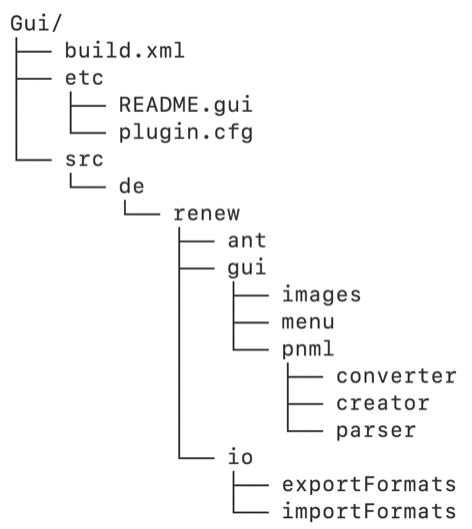
\includegraphics[width=0.4\textwidth]{material/images/gui_struktur.png}
	  \caption{Gui Projekt}
	  \label{fig:gui}
	\end{figure}


	Das Gui Plugin eröffnet die geläufige mangelnde Organisation der Ressourcen. Zum Teil befinden sich diese in den \textit{etc} Verzeichnis und zum Teil sind diese in den Java \textit{source set} im \textit{images} Verzeichnis integriert, wie in der Abbildung \ref{fig:gui} dargestellt.


	Um diese zu beheben, wird das Bild Verzeichnis \textit{de.renew.gui.images}, das mit den \textit{png} und \textit{gif} Daten befühlt ist in das Ressourcen Verzeichnis migriert. Damit die Applikation diese wiederfindet, werden die Zugriffspfade für die Ressourcen innerhalb des Gui Plugin an das neue Verzeichnis angepasst, indem die internen statischen Konstanten , wie \textit{CPNIMAGES}, auf den entsprechenden Ort verweisen. 


	Zum Schluss werden die \textit{README} und die \textit{plugin.cfg}  aus dem \textit{etc} Verzeichnis in das Ressourcen Verzeichnis bewegt. Somit ist eine Struktur erstellt worden, die sich auf das Modulsystem von Java 	anwenden lässt. 
	\bigbreak

	\begin{figure}[h!]
	  \centering
	  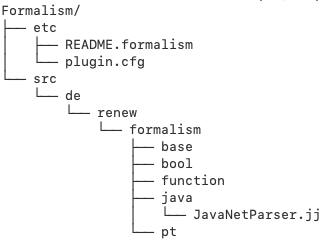
\includegraphics[width=0.5\textwidth]{material/images/formalism_plugin.png}
	  \caption{Formalism Projekt}
	  \label{fig:formalism}
	\end{figure}

	Andere Plugins wie Formalism, CH oder Misc besitzen \textit{JavaCC} Dateien, wie im Beispiel \ref{fig:formalism} dargestellt enden diese auf \textit{jj}. Sie erstellen Java Netz Grammatiken und wandeln die Java-Basis für die Ausführung ab. Diese liegen lose zwischen den Java Klassen und werden von den Java Compiler nicht interpretiert. Daher macht es Sinn diese in ein eigens \textit{Source Set} auszulagern und für den JavaCC Compiler für die Übersetzung zu gruppieren.

	\begin{figure}[h!]
	  \centering
	  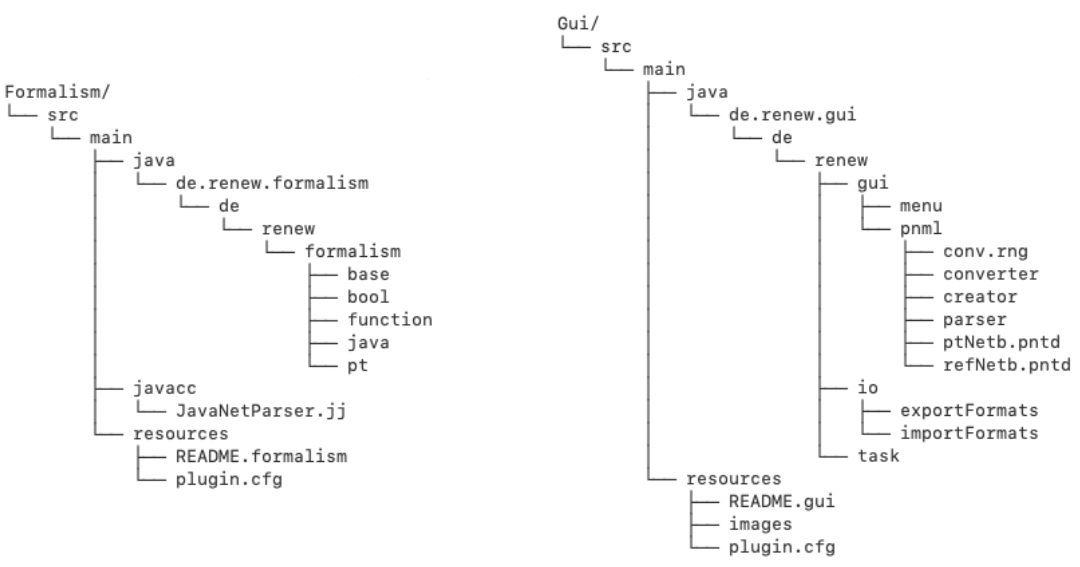
\includegraphics[width=\textwidth]{material/images/form-gui.png}
	  \caption{Resultierende Projektstrukturen}
	  \label{fig:resultStr}
	\end{figure}

	Das Resultat \ref{fig:resultStr} erlaubt eine einfache Paketstruktur Analyse durchzuführen, um die \textit{Split Packages} zu identifizieren. 


	Auf den ersten Blick kann eine Überschneidung zwischen den Gui und den RenewAnt Plugin erkannt werden, da beide den \textit{de.renew.ant} Namensraum besetzen, der sich um bestimmte Ant spezifische Aufgaben kümmert. Aufgrund dessen wird der Namensraum in dem Gui Plugin in \textit{task} zum Gunsten des RenewAnt Plugins umbenannt. Des weiteren könnten beide \textit{Task's} in den RenewAnt Plugin verschoben werden, da dieser keine Abhängigkeiten in dem Gui Plugin besitzt und nicht in den Aufgabenbereich der UI fallen. 

\subsection{Gradle}
 % gradle build script erstellen
 		% Projektstrutur defenieren ()
 		% Klassenpfade für plugin-module und automatischen-module defenieren
 		% Abhängigkeiten Defeneiren und auf den Klassenpfad legen
 		% Subprojekte einbindne über schleifen 
 		% Verärbung der ähnlichen Abläufe wie das compieliren verpacken und bewegen 
 		% Was genau muss ein Unterprojekt besitzen
 		% erst hier wird klar das es keine Zyklen gibt 

 	Um die Zyklen zu erkennen, wird ein Gradle \textit{build} Skript erstellt, der die Java \textit{Source Sets} für den Kompilation Schritt definiert und die benötigten Projekte sowie Drittanbieter-Bibliotheken auf den Projektklassenpfad einbindet. Dafür wird ein übergeordneter Gradle Projekt deklariert, der alle Subprojekte aus allen Plugin Verzeichnissen erstellt. 
	\bigbreak
	\begin{figure}[h!]
	  \centering
	  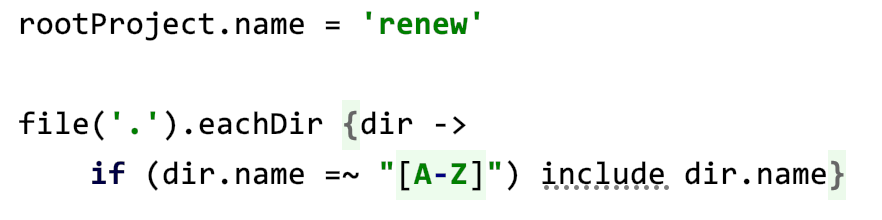
\includegraphics[width=0.6\textwidth]{material/images/settings_gradle.png}
	  \caption{Subprojekte}
	  \label{fig:subprojekte}
	\end{figure}

 	Die \textit{settings.gradle} Datei in der Abbildung \ref{fig:subprojekte}, die in der Konfigurationsphase des Gradle Lebenszyklus ausgelesen wird, ist für diesen Konfigurationsschritt zuständig und kann mithilfe von \textit{Groovy} beliebigen Code für die Deklaration der Projekte enthalten. In diesem Fall werden alle Verzeichnisse, die mit einem Großbuchstaben anfangen als Gradle-Subprojekte eingebunden. 
	\newpage

	\begin{figure}[h!]
	  \centering
	  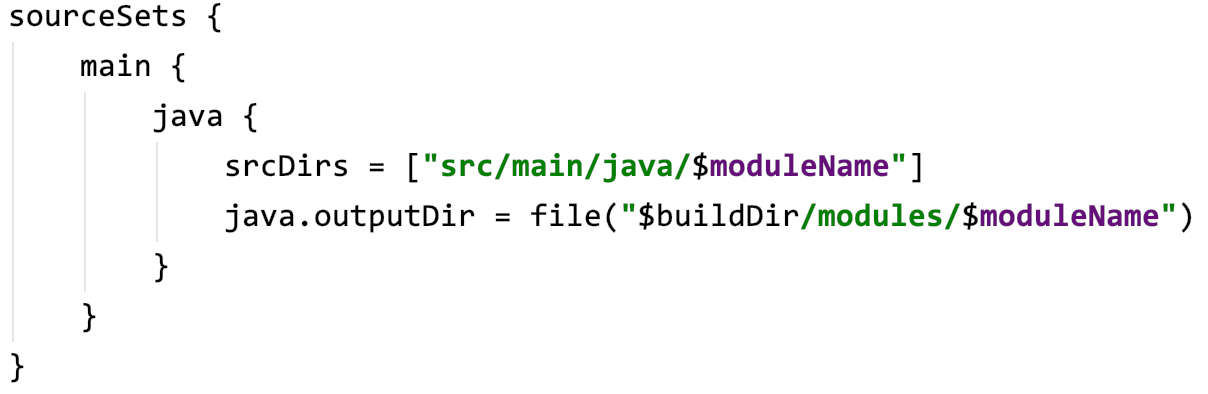
\includegraphics[width=0.7\textwidth]{material/images/sourceSets.png}
	  \caption{Source Sets}
	  \label{fig:Source_Sets}
	\end{figure}

 	Anschließend müssen die Java \textit{Source Sets} des Projekts bestimmt werden. Um die Umsetzung so einfach wie möglich zu gestalten, wird in der \textit{buld.gradle} Konfigurationsdatei, die für die Ausführungsphase zuständig ist, eine \textit{subprojects} Konfiguration angelegt, die für jedes Subprojekte die interne Projektstruktur definieren lässt. Diese beschreibt wo Verzeichnisse mit den Java Code und den dazugehörigen Ressourcen sich befinden sollen.  
	\bigbreak

	\begin{figure}[h!]
	  \centering
	  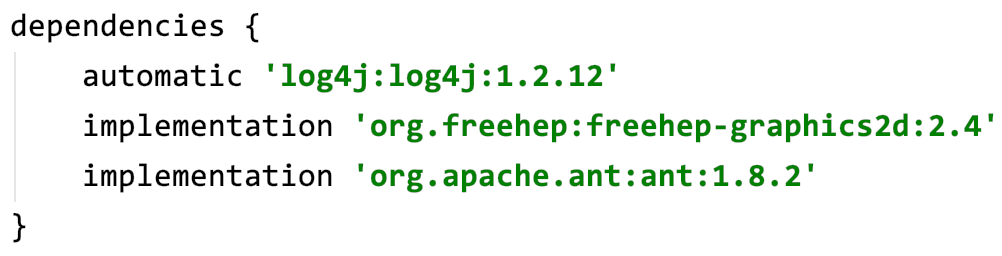
\includegraphics[width=0.6\textwidth]{material/images/dep_global.png}
	  \caption{Drittanbieter-Bibliotheken}
	  \label{fig:deps}
	\end{figure}

 	Im nächsten Schritt werden global genutzte Drittanbieter-Bibliotheken deklariert. Diese werden aus dem \textit{Maven Repository} beim initiiere des Projekts geladen und auf den Klassenpfad aller Plugin Projekte eingebunden. Somit liegt die Verwaltung der Bibliotheken und der dazugehörigen Version an den Maven Repository und muss nicht mehr von uns im GitLab Repository bereitgestellt werden. Die deklarierten Drittanbieter-Bibliotheken in der Konfiguration erleichtern zusätzlich die Aufgabe der manuellen Erstellung der Klassenpfade und die Einbindung der Bibliotheken in der Entwicklungsumgebung, da die Konfiguration von der Entwicklungsumgebung aufgegriffen und auf das Projekt angewandt wird. 
	\newpage

	\begin{figure}[h!]
	  \centering
	  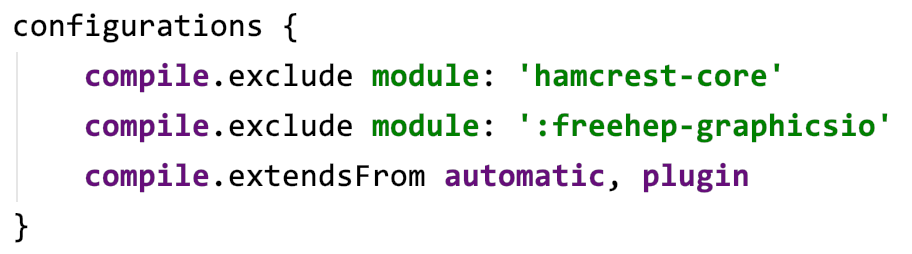
\includegraphics[width=0.6\textwidth]{material/images/configurations.png}
	  \caption{Klassenpfade}
	  \label{fig:kPath}
	\end{figure}

 	Um die Klassenpfade von einander zu trennen werden zusätzliche Konfigurationen mit dem Namen \textit{plugin} und \textit{automaitc} eingeführt, die Plugin Code und Drittanbieter-Bibliotheken von einander trennen und für das Kompilieren zusammenführen. Somit könne diese getrennt von einander Verwaltet, Modifiziert und bei Bedarf für bestimmte Aufgaben angepasst werden. 
	\bigbreak

	\begin{figure}[h!]
	  \centering
	  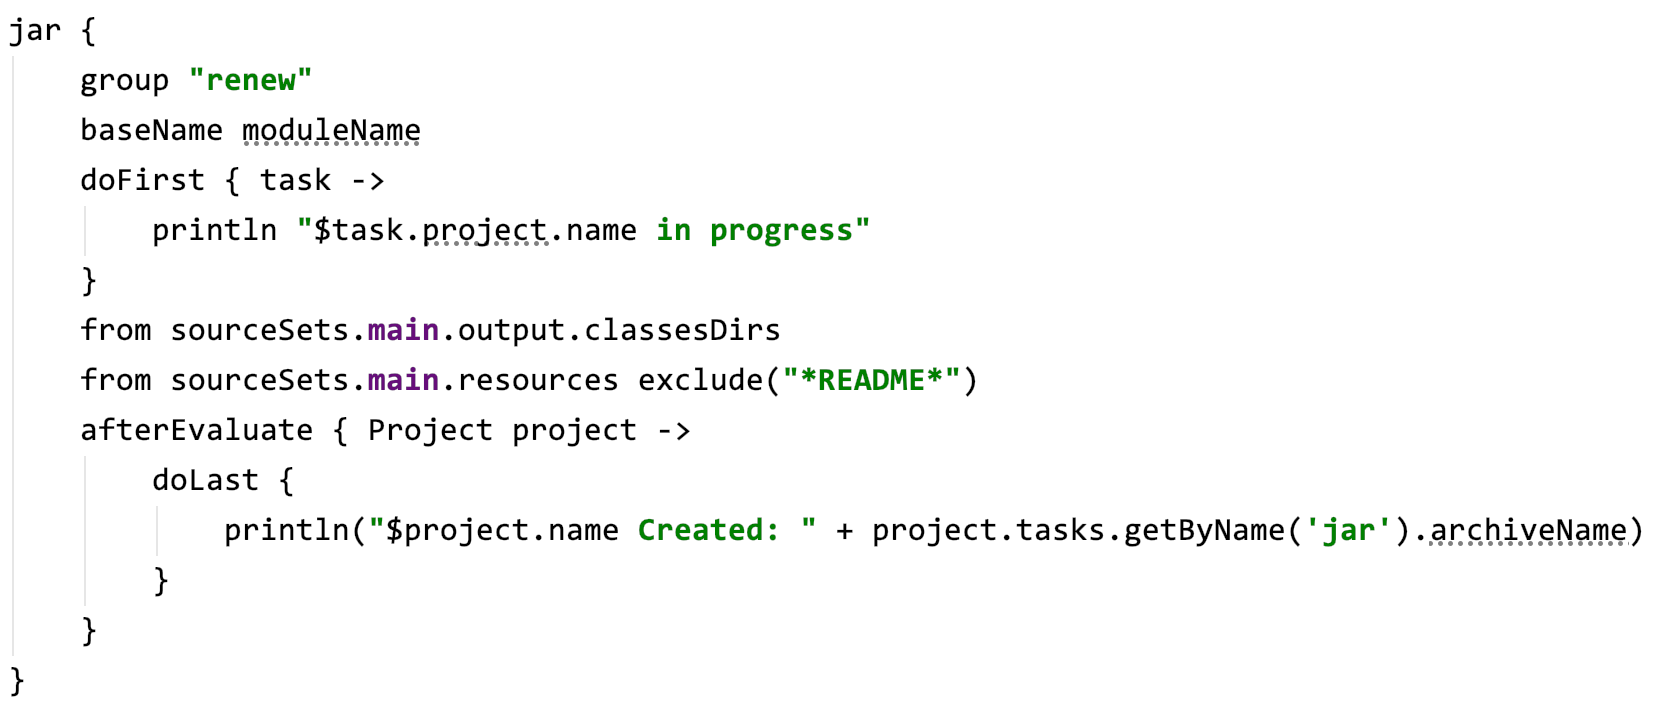
\includegraphics[width=0.9\textwidth]{material/images/jar.png}
	  \caption{Jar Task}
	  \label{fig:jar}
	\end{figure}

	Zum Schluss der globalen Konfiguration wird ein \textit{jar} Task angelegt, der für ein gegebenes \textit{Source Set} ein \textit{jar}-Archiv für jedes Plugin mit den dazugehörigen Ressourcen erstellt. 


	Damit ist die globale Konfiguration der Renew Plugins beendet und bereit für die individuelle Anpassung der Plugin Bedürfnisse.
	\bigbreak

	\begin{figure}[h!]
	  \centering
	  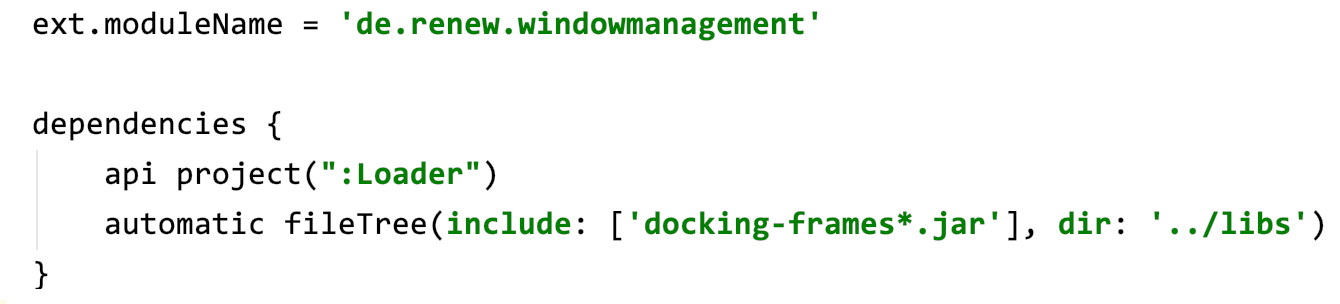
\includegraphics[width=0.8\textwidth]{material/images/windmang.png}
	  \caption{Individuelle Konfiguration}
	  \label{fig:windmang}
	\end{figure}

	Die Plugins benötigen einen internen Namen für die Verwaltung und die zusätzlichen Drittanbieter-Bibliotheken sowie Plugin Abhängigkeiten. Dafür wird in der Plugin \textit{buidl.gradle} Konfigurationsdatei der Name unter den \textit{extension properties} deklariert und die bereits geerbten Abhängigkeiten erweitert. In der Abbildung \ref{fig:windmang} wird das WindowManagment Plugin durch eine lokale, modifizierte Drittanbieter-Bibliotheken  und durch das Plugin Projekt erweitert, um alle Benötigen Abhängigkeiten abzudecken. 
	\bigbreak


	Jedes einzelne Plugin wird auf diese Weise konfiguriert und enthält einen Namen sowie zusätzliche Abhängigkeiten. Hiermit ist die Vorbereitung für die Modularisierung abgeschlossen. 


\subsection{Modularisierung}	
	Nachdem alle benötigen Renew Plugins kompiliert, verpackt und ausgeführt werden können, müssen die neu entstandenen Abhängigkeitsbeziehungen analysiert werden. Die Analyse der Plugins geschieht nun über die erstellten Gradle Scripte, die für jedes Projekt die benötigten Bibliotheken und Projekte für die Kompilation definieren. Aus diesen wird ein Abhängigkeitsgraph erstellt, der Zyklen und versteckte Abhängigkeiten offenlegt. 
	\bigbreak

	\begin{figure}[h!]
	  \centering
	  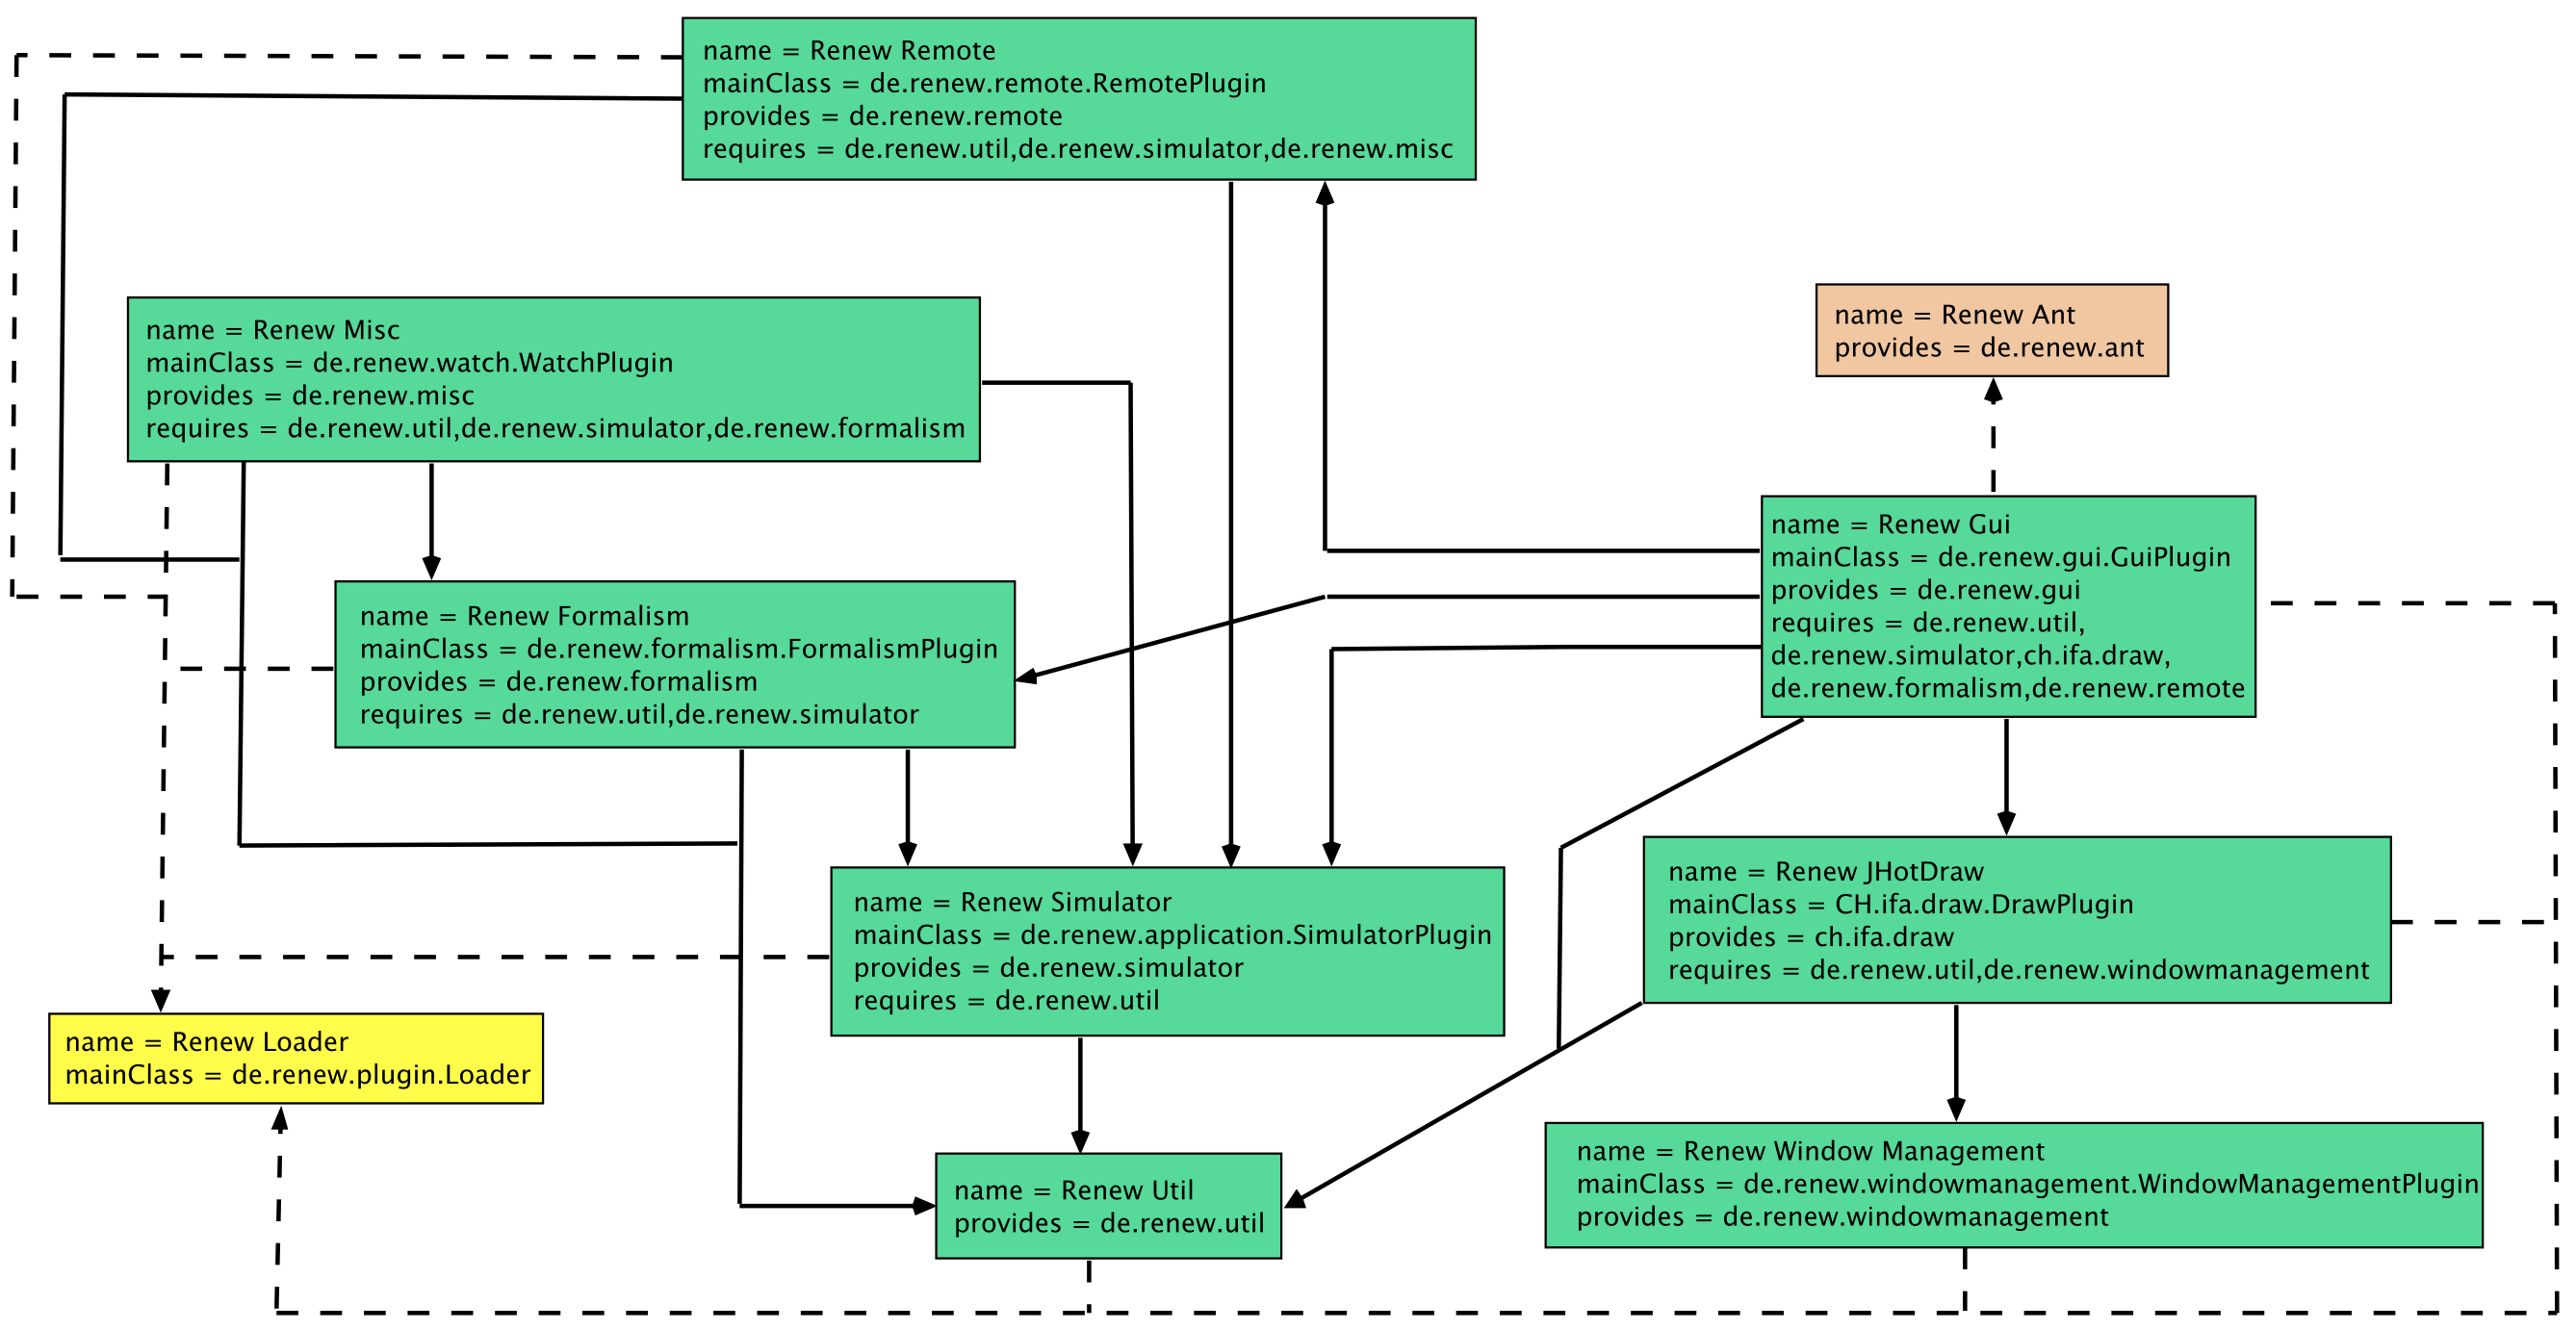
\includegraphics[width=\textwidth]{material/images/deps_tree.png}
	  \caption{Kompilation Abhängigkeiten}
	  \label{fig:deps}
	\end{figure}

	Der neu entstandenen Graph wurde im Vergleich zu dem Graphen aus dem Ausgangssituation Abschnitt \ref{fig:plugin_deps} durch ein Plugin erweitert und bindet alle Plugins an das \textit{Loader} Projekt. Des weiteren sind auf der Abbildung \ref{fig:deps} keine Zyklen in der minimalen Version zu beobachten und dementsprechend müssen auch keine weiteren Anpassungen durchgeführt werden. 
	\bigbreak

	Die Migration von der minimalen Version von Renew wird von den \textit{Loader, Util} und \textit{Windowmanagment} Plugin eingeleitet. Diese besitzen keine Abhängigkeiten innerhalb der Plugin Menge und brauchen keinen Zugriff auf den Klassenpfade nachdem sie sich auf dem Modulpfad befinden. Im Gegensatz dazu, behalten Plugins, die sich auf dem Klassenpfad befinden und als ein unbenanntes Modul interpretiert werden, alle Zugriffsrechte auf die interne Struktur migrierten Plugins, wie bereits in den Abschnitt \ref{fig:modacc} beschrieben wurde.
	\bigbreak

	Da ein Modul seine eigne Abhängigkeiten verwalten muss, wird für jedes Plugin eine \textit{module-info.java} Konfigurationsdatei angelegt, die alle Java internen sowie Drittanbieter Bibliotheken auflistet. Für die ersten Module werden die erforderlichen Bibliotheken inklusive dem Loader Plugin in der Konfigurationsdatei mit dem Schlüssel \textit{requires} verankert und die dazugehörigen Drittanbieter-Bibliotheken aus den Klassenpfad auf dem Modulpfaden als automatische Module aufgesetzt.
	\begin{figure}[h!]
	  \centering
	  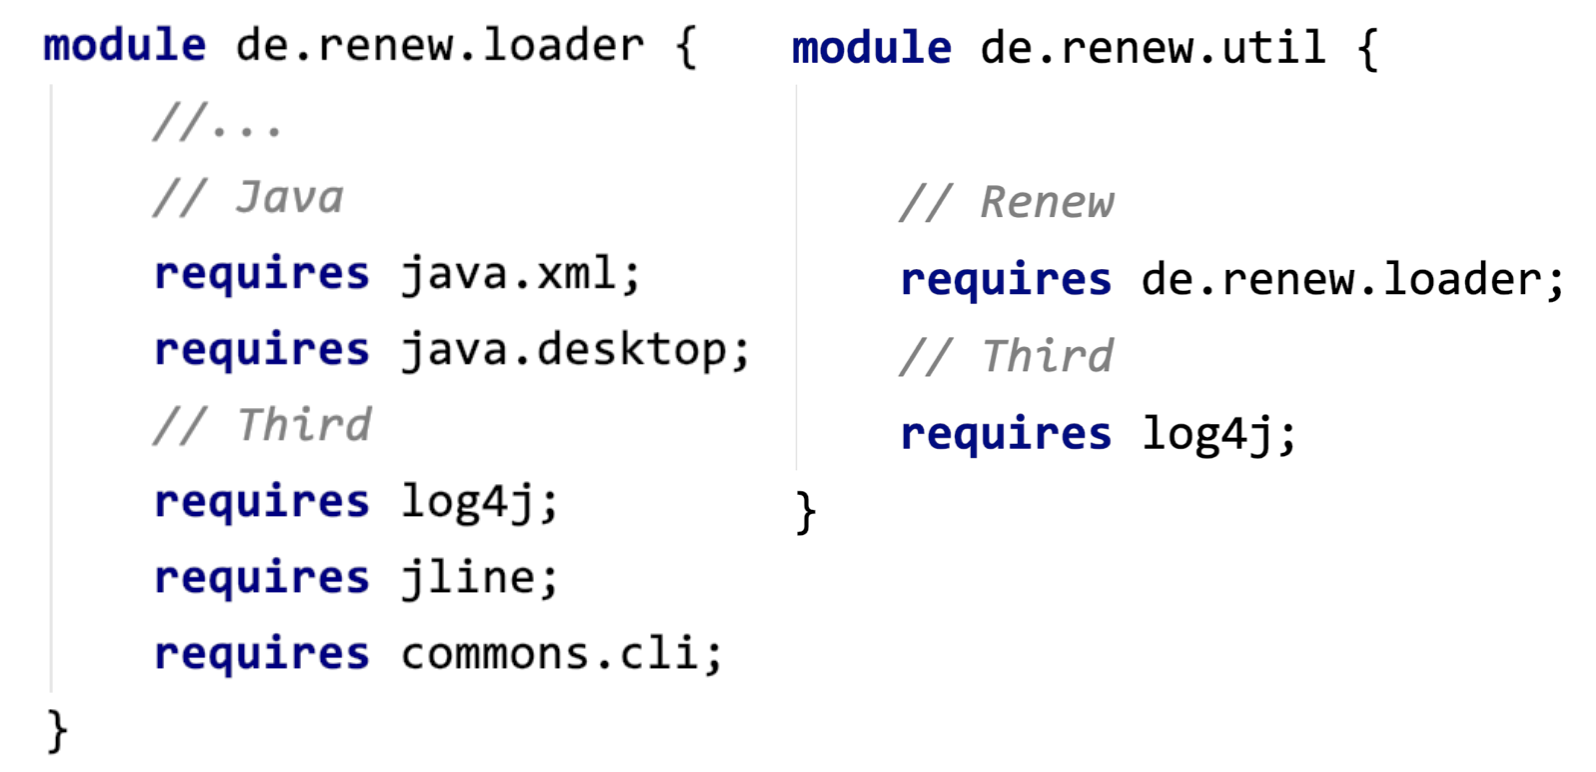
\includegraphics[width=0.7\textwidth]{material/images/loaderUtil-info.png}
	  \caption{Module Infos}
	  \label{fig:loaderUtil}
	\end{figure}

	In diesem Zustand wird Renew kompiliert und ausgeführt. Das Ergebnis ist eine lauffähige Applikation, die identisch zu der initialen minimal Version von Renew funktioniert. 
	\bigbreak

	Im nächsten Schritt werden Plugins migriert, die nur auf die neu entstandenen Module aufsetzen, wie zum Beispiel das \textit{Simulator} und das \textit{JHotDrow} Modul. Ihre Abhängigkeiten liegen auf dem Modulpfaden, daher gibt es keinen Grund mit dem Klassenpfad zu interagieren. 


	Da diese die zweite Modulschicht repräsentieren, fordern sie bestimmte Funktionalität mit dem \textit{requiers} Schlüssel aus den Loader, Util und Windowmanagment Plugins. Um diese Anforderung zu entsprächen, müssen die notwendigen Plugins ihre Pakete  explizit für ihre Nutzer öffnen. Dazu deklarieren die angeforderten Plugins in ihrer \textit{module-info.java} mit dem \textit{exports} Schlüssel Pakte, die sie für andere Plugins zur Verfügung stellen möchte. 
	\begin{figure}[h!]
	  \centering
	  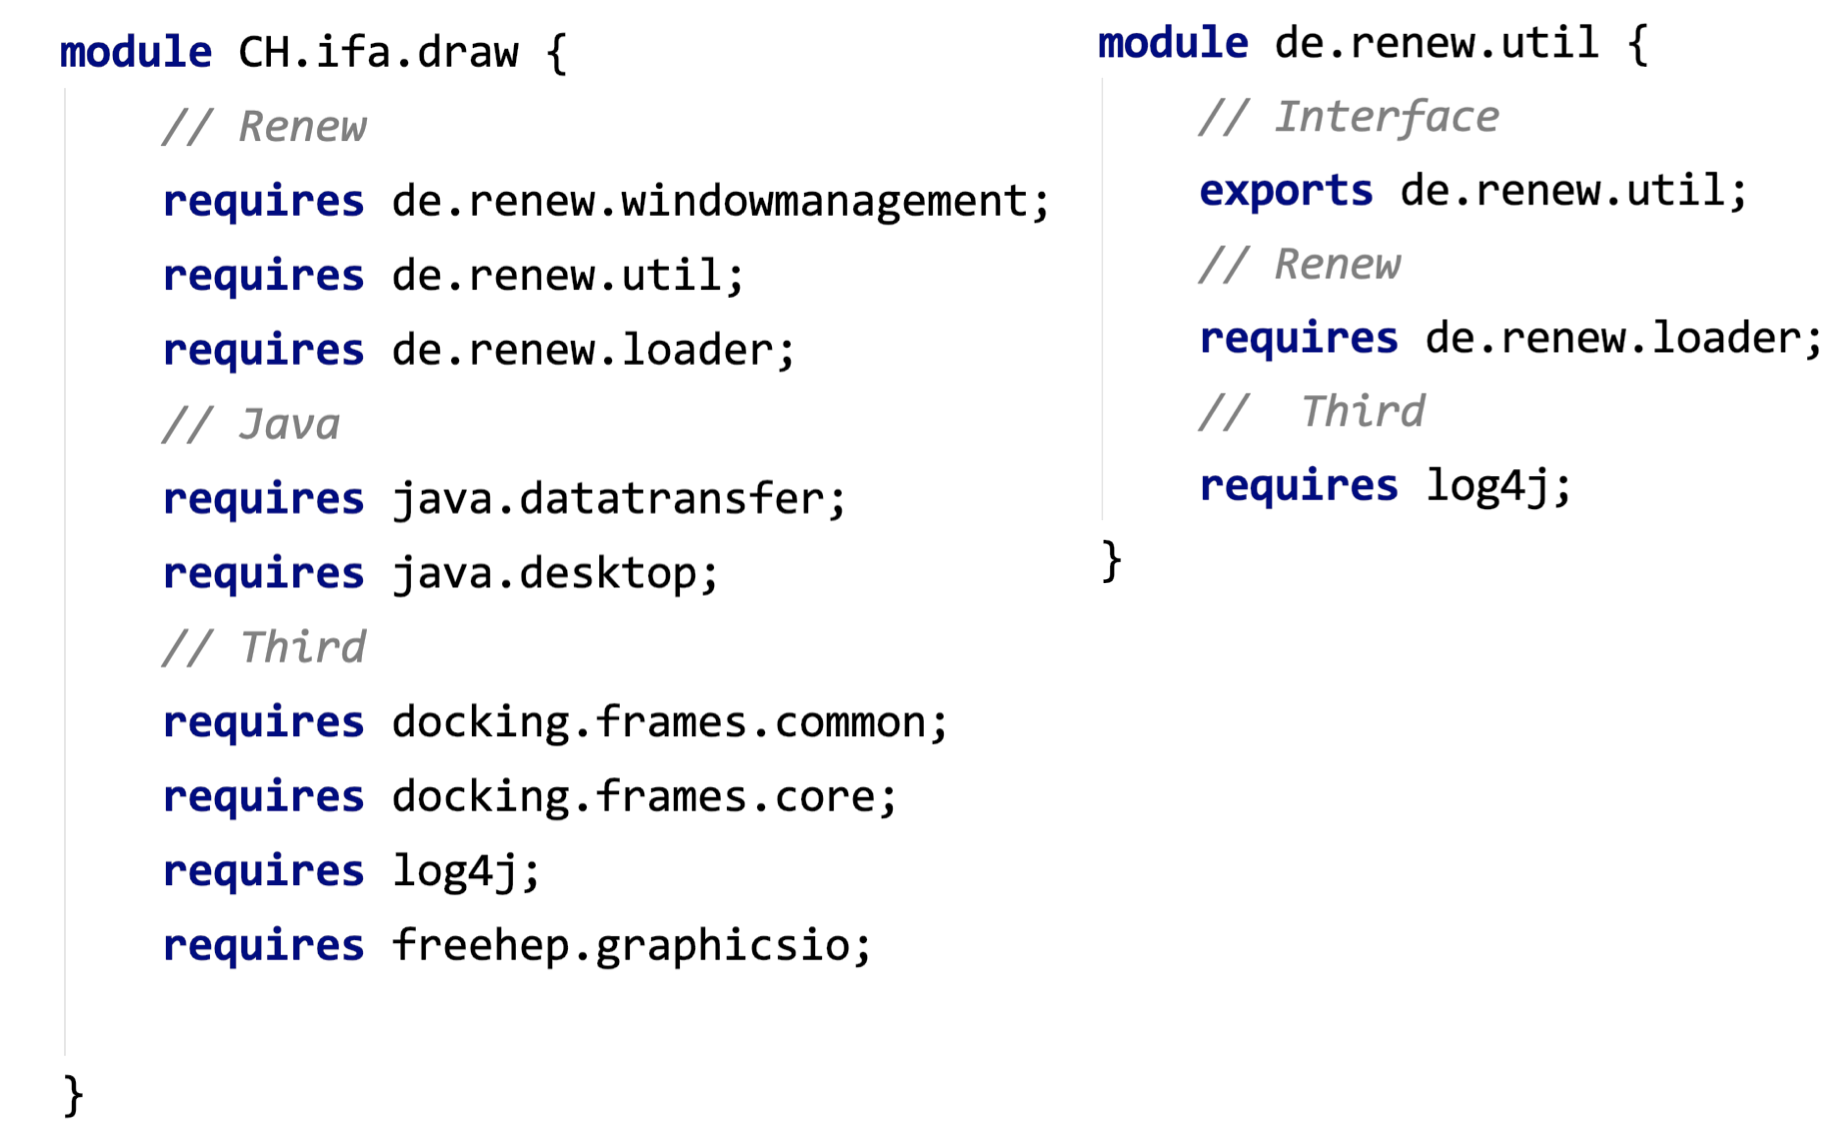
\includegraphics[width=0.8\textwidth]{material/images/utilCH-info.png}
	  \caption{Module Infos}
	  \label{fig:utilCH}
	\end{figure}

	In der Abbildung \ref{fig:utilCH} wurde das Util Plugin Modul angepasst und bietet jetzt das \textit{de.renew.util}  Paket für den Gebrauch an. 
	\bigbreak

	Die Adaption der bestehenden Module muss mit jeder neuen Modulschicht an die angeforderten Pakete und Klassen angepasst werden, bis alle Abhängigkeiten erfüllt sind. 


	Damit sind die notwendigen Schritte für die Modularisierung bestimmt worden und können in einem Zyklus, bis alle Plugins auf dem Modulpfaden befinden, durchgeführt werden. Nähmilch das Auslesen und Definieren der Plugin Kompilation- sowie Laufzeit Abhängigkeiten aus dem Gradle Build Skript mit dem Schlüssel \textit{requires} und das Nachrüsten der Schnittstellen bestehender Module mit dem \textit{exports} Schlüssel. 
	\bigbreak

	Auf der Nächsten Seite in der Abbildung \ref{fig:migration} wird die komplette Migration in vier Schritten dargestellt.


	\begin{figure}
	  \centering
	  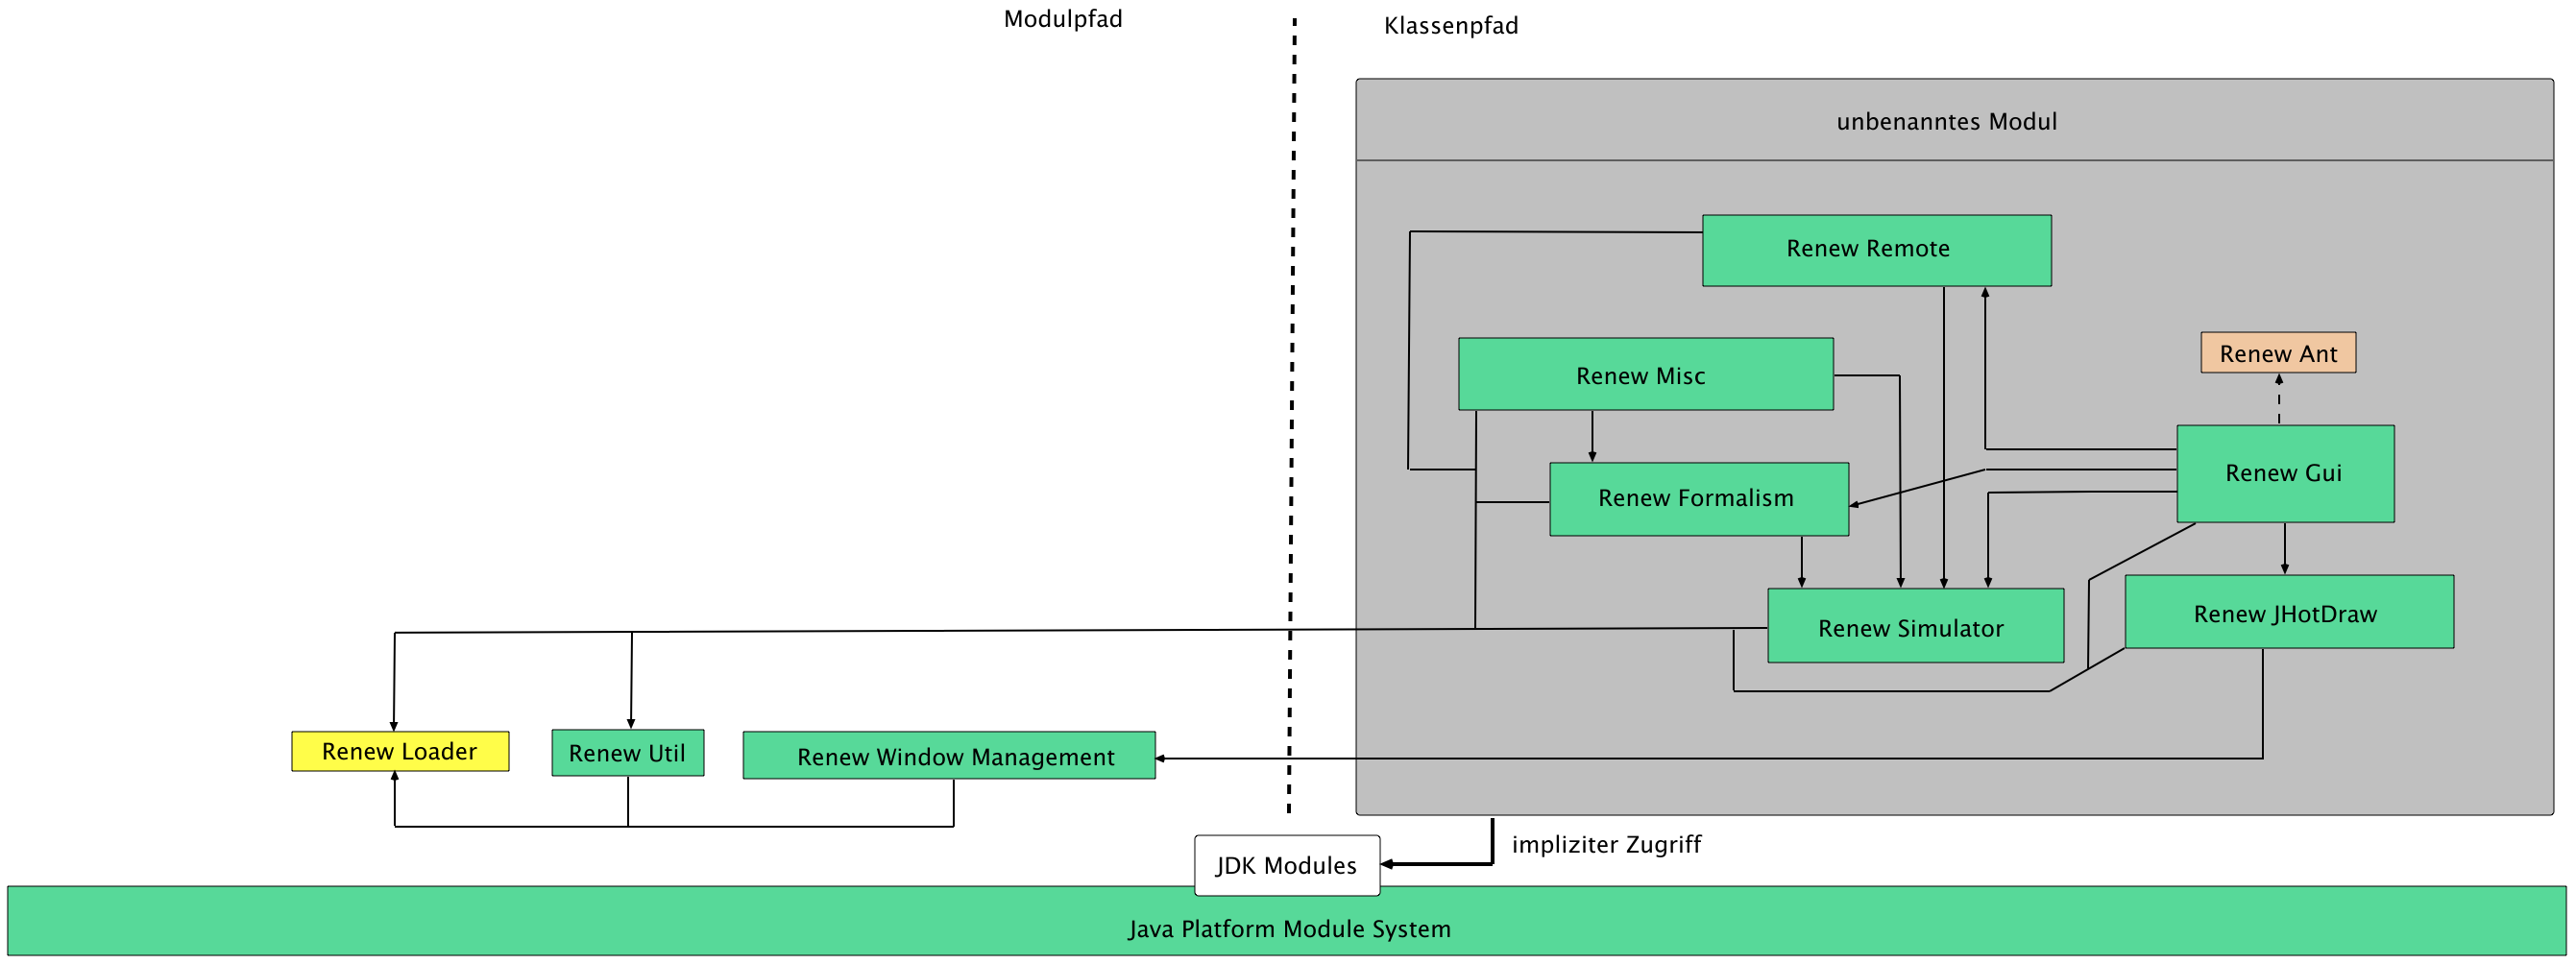
\includegraphics[width=\textwidth]{material/images/1step.png}
	  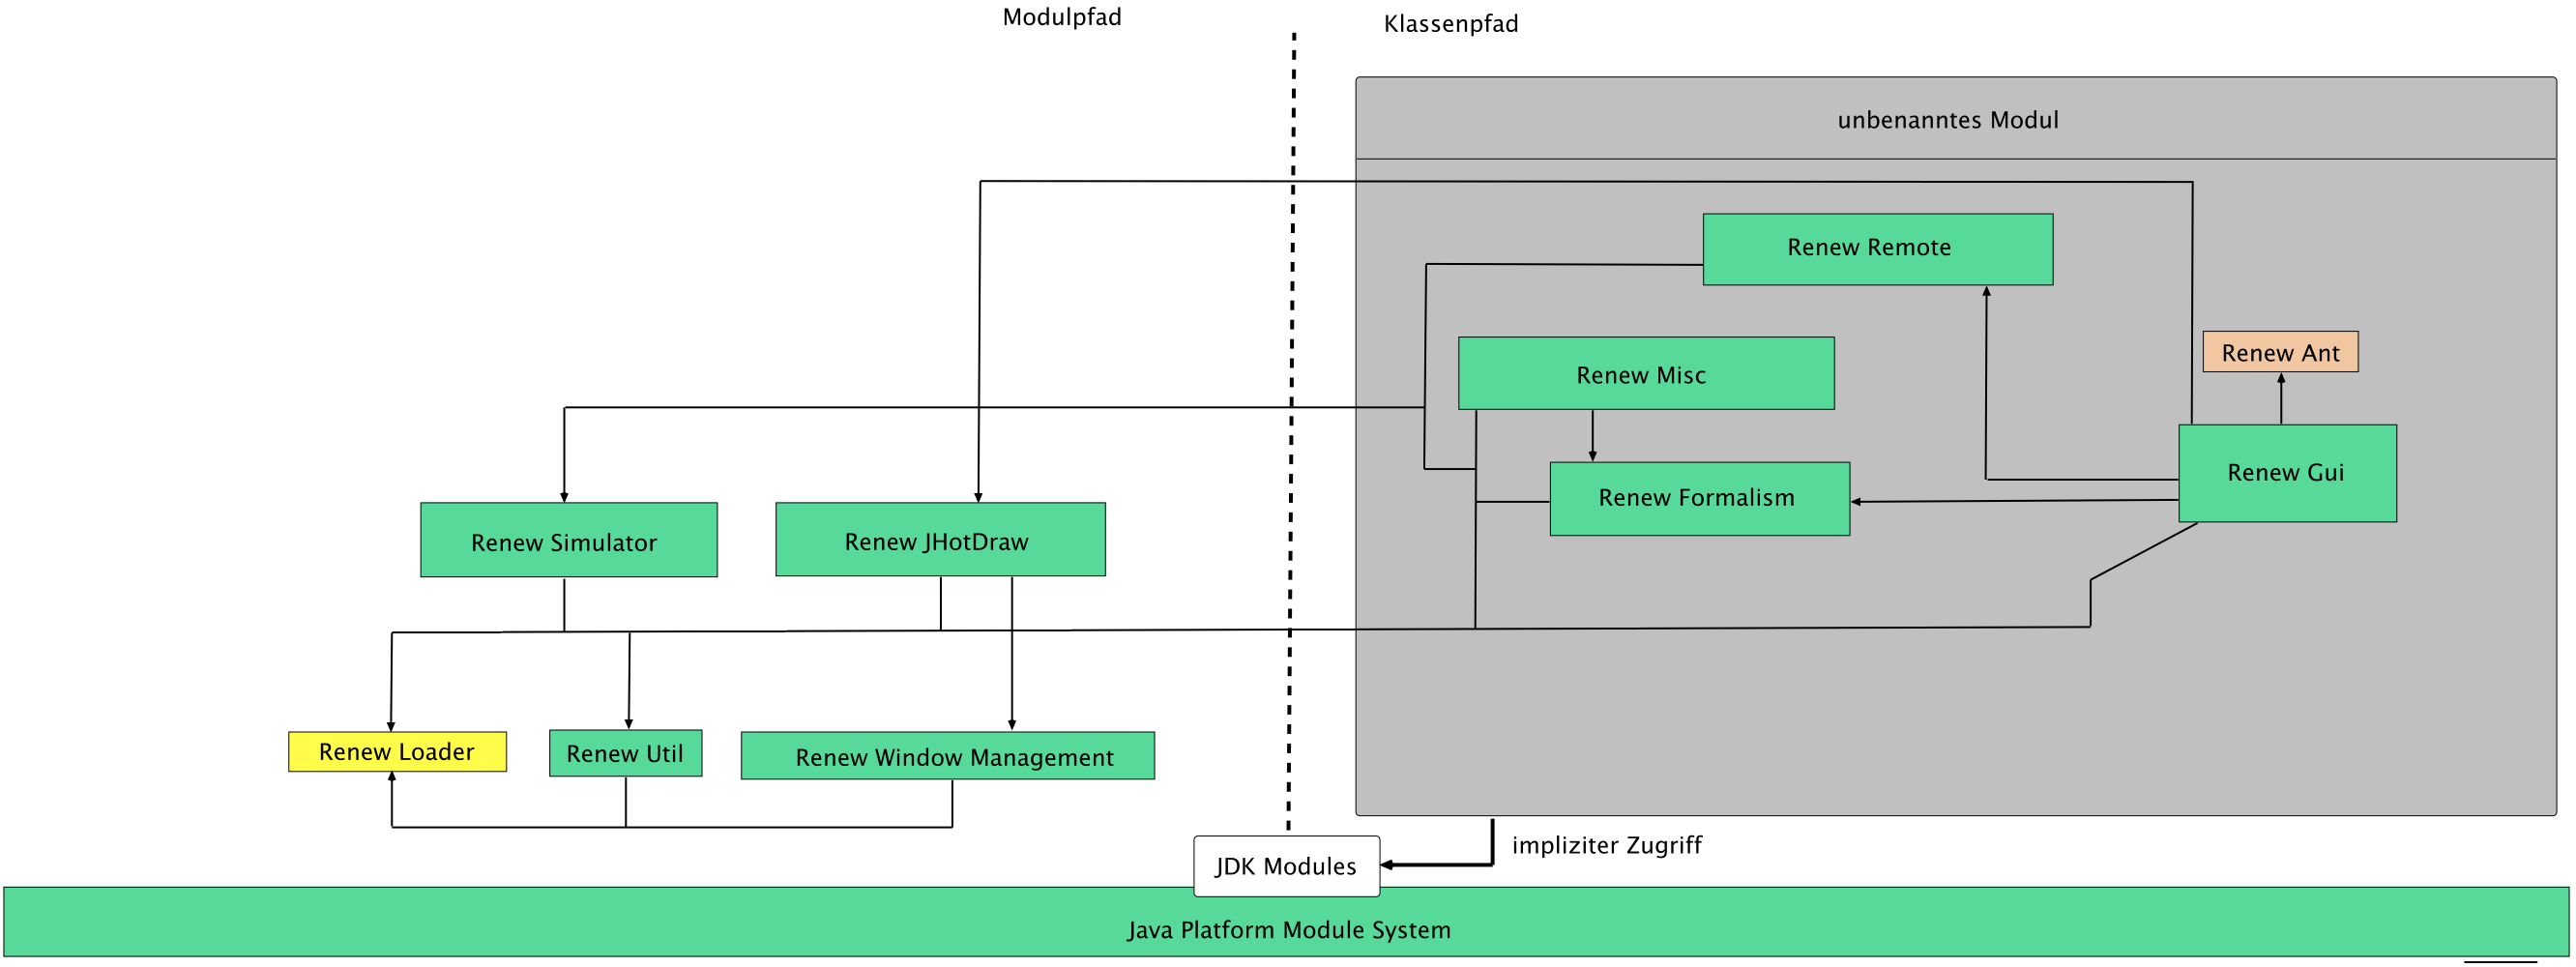
\includegraphics[width=\textwidth]{material/images/2step.png}
	  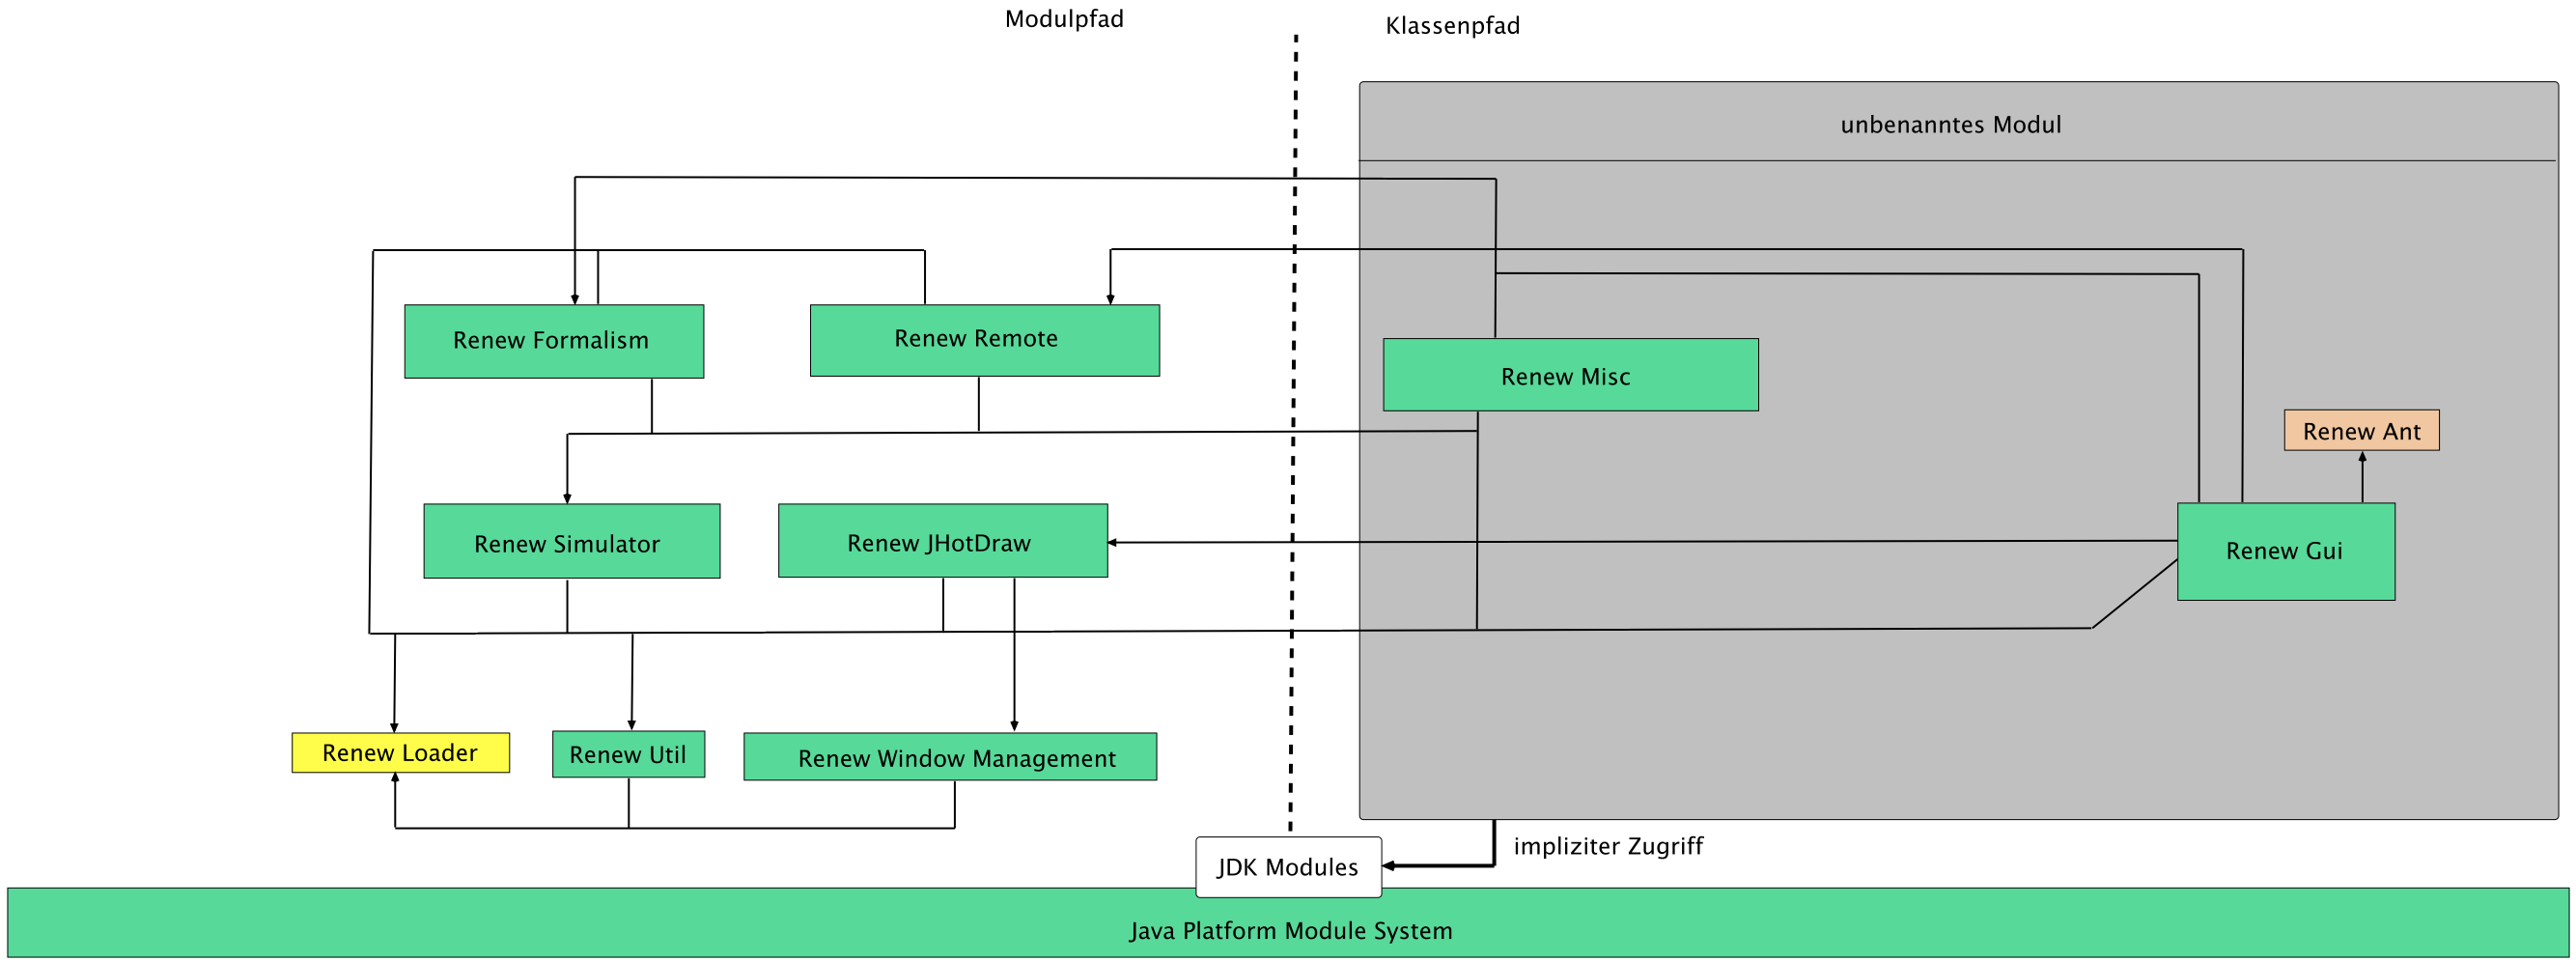
\includegraphics[width=\textwidth]{material/images/3step.png}
	  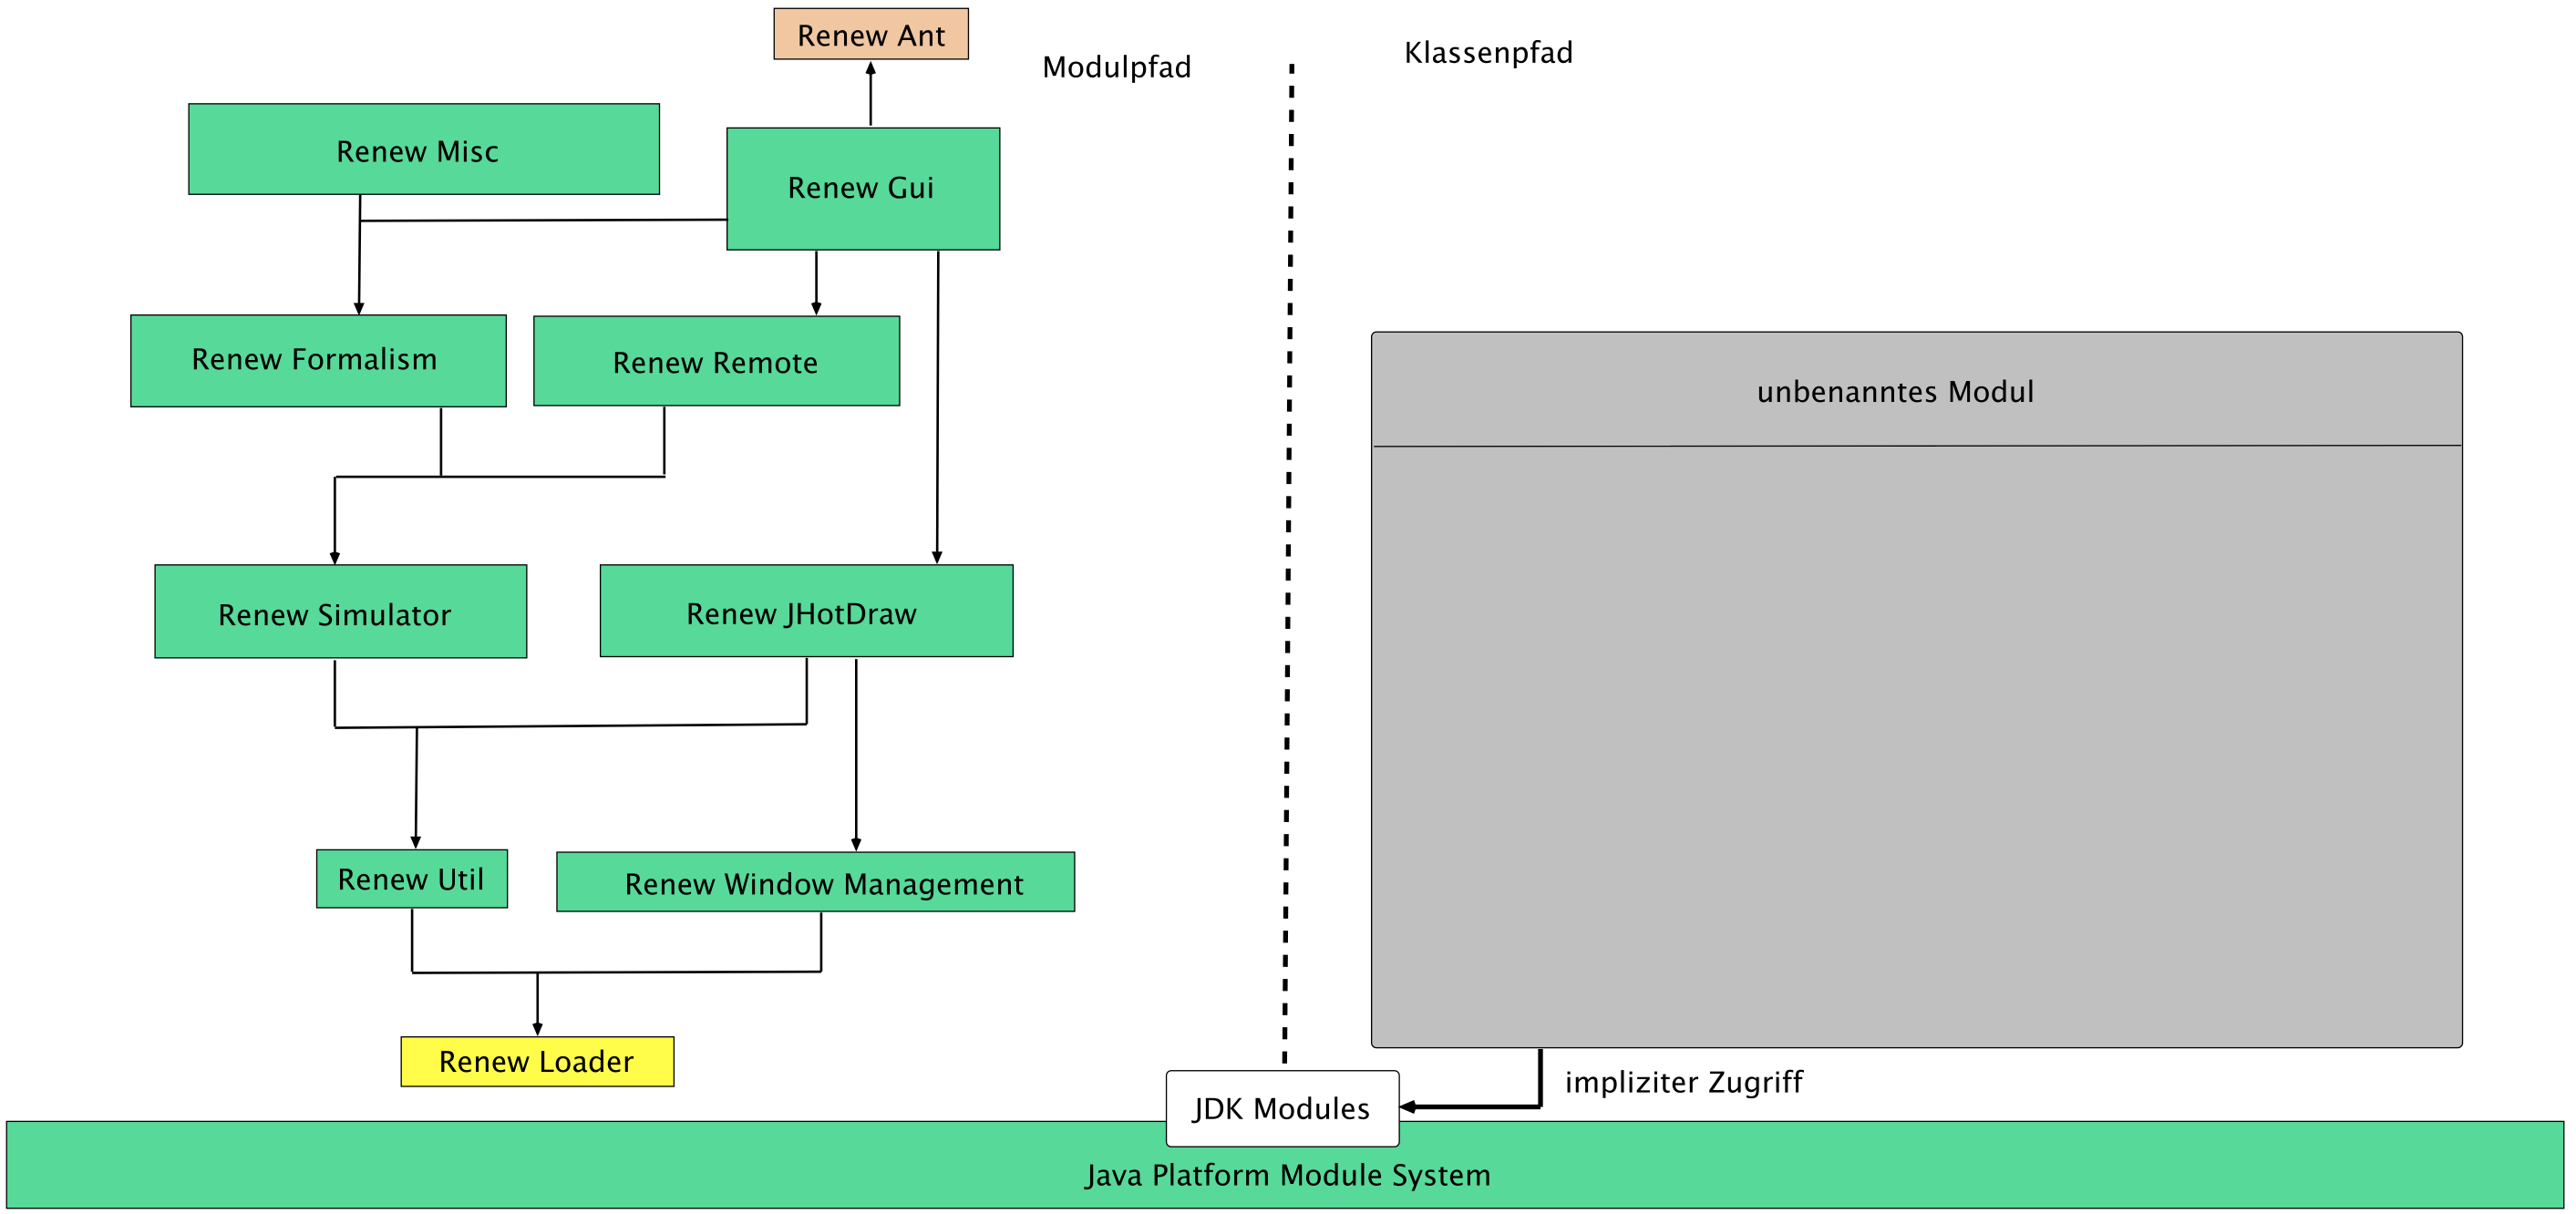
\includegraphics[width=\textwidth]{material/images/4step.png}
	  \caption{Migration}
	  \label{fig:migration}
	\end{figure}	

\section{Evaluation}

% Projektstruktur: tolle sache zusätzlich für da stesten kännten die tstrs sachen richtig eingegleiderst werden 

% Gradel: Vergleichen der Code Zeile in Ant und Gradle

% Modularisierung: Pluginarten wie compile, runtime mit der static Abhängigkeiten. RenewAnt 

% Modularisierung: Simple Umsetzung der Abhängigkeiten imt transitiv 

% Gradel: unterstützt die modualre idee mit api und  implemetnation 



% Auscheken des projekts schneller da drittanbieter nicht mitgezogen werden müssen. Versionsverwaltung ist einfacher mit nur einem Character Anapssung 

% Trennen der Klassenpfade hilft die Struktur zu verwalten automatic runtime compoe api und implimentation 

% JavaCC aus allen Plugins in einem gemeinsamen Plugin zusammenfassen 



 
 % testsrc -> test viel besser 
% javacc ausgelagert 
% ant tasks komplet im ant plugin verwalten ?
% Was hat gradle besser als gedacht umgesetzt, wieso ist es toll "teaser"

 % git Drittanbieter-Bibliotheken schwer und brauchen platz jetzt nicht mehr. 
 % git Versionsverwaltung einfach 
 % vorteil von trennen der Klassenpfade automatic pluign
 % ant sachen alle nach ant verschieben und über export zugreifen ???
 % Abgleich mit Ant build script in Zeilen, Komplexität und erweiterbarkeit (Oder in der Evaluation)
 % eine Anforderungsmenge die von mehreren Prototypen umgesetzt wird 


% Dafür wir diese von dem Rest des Systems isoliert und auf Kompilation sowie Laufzeit Abhängigkeiten untersucht. $